\section{Methods}
\label{sec:methods}

For all statistical significance tests, a significance level of $0.05$ was assumed.

\subsection{Overall measurements of negative affect and its variability}

As proposed in \citet{rutter2024}, one way of estimating negative affect levels and variability is, to simply aggregate all observations for an individual to compute a single score for them. Thus, for investigating NA levels, one takes the arithmetic mean of all NA scores for a person and for NA variability one takes the standard deviation of all NA scores for that person.

This yields an overall NA level $x_i$ and an overall NA variability $\sigma_i$ for each person $i$. Then, let $A$ be the set of anxiety patients and $D$ the set of depression patients. 

Then, the separate overall mean NA level scores are

\begin{equation}
    \bar{x}_a = \frac{\Sigma_{i = 1}^{n} x_i}{n}, n := |A|
\end{equation}

for the A cohort and 

\begin{equation}
    \bar{x}_d = \frac{\Sigma_{i = 1}^{n} x_i}{n}, n := |D|
\end{equation}

for the D cohort. Similarly, the separate overall mean NA variability scores are

\begin{equation}
    \bar{\sigma}_a = \frac{\Sigma_{i = 1}^{n} \sigma_i}{n}, n := |A|
\end{equation}

for the A cohort and 

\begin{equation}
    \bar{\sigma}_d = \frac{\Sigma_{i = 1}^{n} \sigma_i}{n}, n := |D|
\end{equation}

for the D cohort.

Then, one can compare the two means and make inference regarding the differences on the population level by testing the null hypotheses

\begin{equation}
    H_{0V} : \bar{\sigma}_a = \bar{\sigma}_d
\end{equation}

and

\begin{equation}
    H_{0L} : \bar{x}_a = \bar{x}_d.
\end{equation}

\subsection{Localized measures of negative affect and its variability}

In order to obtain localized measures of negative affect magnitude and variability, indicators were computed in rolling windows across the time series. Thus, for each individual, there was not just one overall affect level, but instead one for each smaller time period. After obtaining these mean NA levels for each window, the aggregated scores from all windows for an individual were further aggregated. For assessing NA levels, they were again averaged, while the standard deviation of these scores represents the overall NA variability for an individual. The window construction is illustrated in Figure \ref{fig:windowing}

The first window size option was a 6-hour window. We aimed to capture a more stable estimation of short-term affect levels. The threshold of 6 hours was chosen because it is not too short where it would merely capture single tweets, but also short enough in order to capture short-term affect levels. Each observation served as the center of a window exactly once. Thus, for each observation in the dataset, a window of three hours before and three hours after the observation was created and the NA levels were aggregated using the arithmetic mean in order to obtain a window score. If only one observation was contained in a window, the window centered around it was omitted for all analyses. 

The second window size that was tested is a daily aggregation. For this, all observations for a person from a single calendar day were aggregated. We assumed that users' NA levels do not just fluctuate during the day, but also between days. This aimed to operationalize the idea of "good" and "bad" days. Thus, we obtained a single NA score for each calendar day, represented by the mean NA score of all tweets on that day.



\begin{figure}[h]
    \centering
    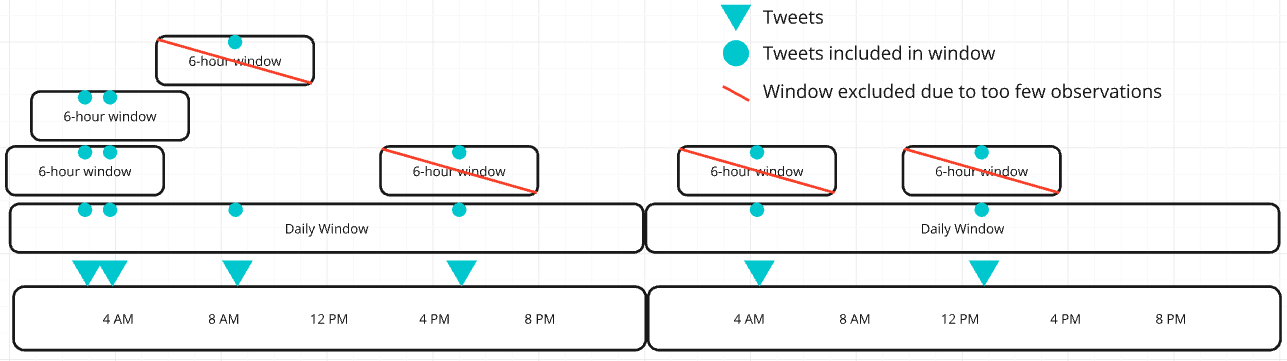
\includegraphics[width=\linewidth]{Images/windowing.png}
    \caption{Construction of windows on tweets of a single individual}
    \label{fig:windowing}
\end{figure}

\subsection{Validity of application of simple aggregation functions}

For windowed analyses, all observations for a person within a certain time window (which yield a distribution of NA values) were aggregated to a single number. For NA levels, the arithmetic mean was used, while NA variability was measured by standard deviation. These measurements, albeit simple, put some assumptions on the data that required investigation. 

First, the mean of a distribution always gives the average value of all observations, can be inflated by outlier observations quite easily though. Therefore, its interpretation can change for skewed distributions because there no longer is such a clear center of the distribution as in a symmetric one. The mean $\bar{x}$ of a sequence $X$ is defined as 

\begin{equation}
    \bar{x}= \frac {1}{n} \sum _{i=1}^{n}x_{i},
\end{equation}

while the sample standard deviation $\sigma$ is

\begin{equation}\sigma
 = \sqrt\frac{\sum{(x_i-\bar{x})^2}}{n-1}.
\end{equation}

It becomes clear, that $\sigma$ depends on $\bar{x}$ and therefore has the same interpretation assumptions. It follows, that the standard deviation is a measure of symmetric spread around the mean and also suffers from the same susceptibility to outliers that the arithmetic mean suffers from.

Whether this is a good measure of aggregation depends on a few facts about the distributions. Figure \ref{fig:suitability_mean} shows three types of distribution that have very different characteristics.

\begin{figure}[h]
    \centering
    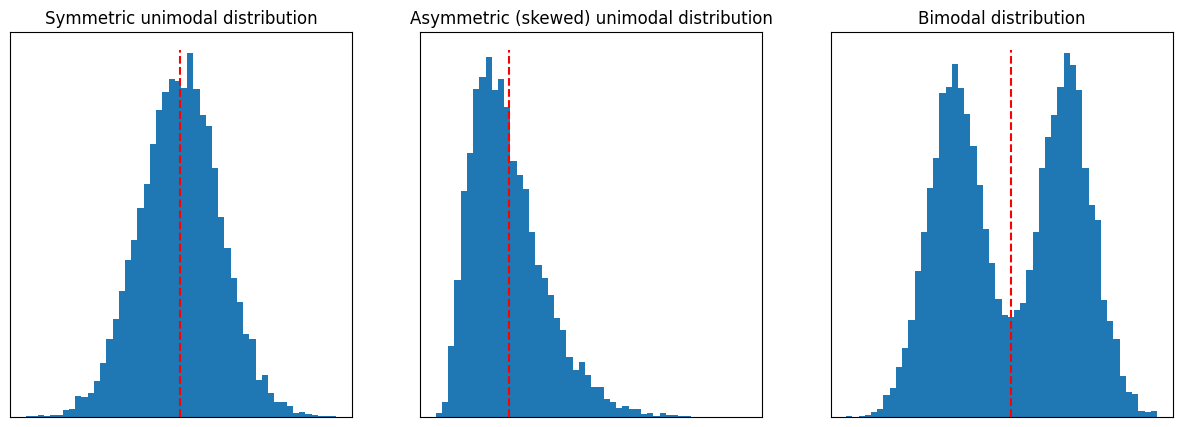
\includegraphics[width=\linewidth]{Images/suitability_of_mean_agg.png}
    \caption{Visualization of placement of arithmetic mean (red dashed lines) for different types of distribution}
    \label{fig:suitability_mean}
\end{figure}

First, the symmetric unimodal distribution can be summarized quite well using an arithmetic mean (as indicated in the figure). In this case, the mean, mode and median are all approximately equal. Also, its standard deviation gives a very good estimate of spread, because the observations are evenly spread around the mean. This is because the standard deviation is approximately just the mean squared deviation from the sample mean and therefore symmetric.

Second, the asymmetric, or skewed, distribution shows a different behaviour. In this case, the mean is not at the peak of the distribution (mode), indicating that it is not necessarily the perfect means of assessing location of the distribution. One could debate here, whether the mean is what we intend to measure or whether one is rather interested in the mode of the distribution.

Third, the bimodal distribution represents an entirely separate challenge. It is (in the case from Figure \ref{fig:suitability_mean}) made up of two symmetric unimodal distributions that are displaced by some offset. In this case, if both distributions are equal in spread and simply placed at different points on the x-axis, the placement of the mode of this distribution is simply a random coin toss between the two modes of the underlying distributions. The mean will always measure some point in between both modes. In this case, one could argue that neither the mode, nor the mean, nor the median is a good measure of location, because the distribution is likely not one, but multiple that might even be separable by some criterion.

Because the quality and interpretation of the aggregation of observations for a person within a window depend so much on the kind of underlying distribution, we had to investigate the distributions. Since the ideal case (in which the mean is basically a perfect measure of NA level) is the symmetric unimodal distribution, a test was performed in order to check whether this assumption holds. 

For this test, all means and medians of these distributions (for one person, for one window) were gathered and compared using a pair-wise t-test for dependent samples. This tests the means and medians for equality. If they are unequal, there must be some systematic skewedness in the data, indicating that the applicability of the mean and standard deviation as aggregation measures is debatable.

The results of this analysis showed, that for the raw data ($t(1301) = 106.68; p < .001$), the 6-hour windowed NA levels ($t(1298) = 32.72; p < .001$) and the daily aggregation ($t(1301) = 37.17; p < .001$), the assumptions were violated. Thus, there is reason to believe that mean and standard deviation were not an optimal measure of location or spread of the NA distribution. 

\subsection{Group comparisons with localized measurements}

As described, all window aggregations for a person were aggregated to obtain a single score for a person. This score was either the mean (for NA level comparisons) or the standard deviation (for NA variability comparisons) of windowed NA levels. Thus, each participant was represented by a single value on both dimensions (NA level and NA variability).

With these scores for each individual, they were again split into anxiety and depression cohorts. Then, the two samples were compared with respect to their means using Mann-Whitney-U tests. Thus, for NA level comparisons, the mean NA levels for each user were compared, while the mean standard deviation was compared for NA variability. The obtained test statistic was tested for statistical significance and used for inference.

\subsection{Analysis of negative affect differences using linear mixed models}

In addition to the overall and windowed aggregations of NA levels and NA variability, we introduce a new method for inferential statistics. Here, linear mixed models (LMM) were used to model the correlation between NA scores and a set of predictor variables. In this approach, NA level differences as well as NA variability differences between the cohorts can be extracted from a single process.

The assumption that underlies this method is, that the lower the affect variability, the easier it should be to predict the negative affect level at a given time. So, in order to test whether there are differences in variability between cohorts, the residual variances of a predictive regression model can be compared. If one cohort has higher residual variance than another, one can conclude, that the affect levels are more difficult to predict and therefore higher in variability.

With this method, one can estimate the differences in variability that are not simply due to external factors, but seemingly unexplainable. This is because one can include external factors in the form of covariates in the model specification, yielding a more robust estimation of variability differences.

The dataset consisted of repeated measures of sentiment (VADER NA score) for multiple users over time, alongside other covariates (user-level features). Since sentiment was tracked across time, the dataset was inherently longitudinal, where series of observations are nested within individuals.

In this type of data, several key challenges arise. One challenge is correlation within subjects. Repeated observations of the same user are not independent. Responses (VADER scores) for a given user are likely correlated over time. Failing to account for this correlation may lead to biased standard errors and incorrect inference. 

Another challenge is that users can be quite heterogeneous with regards to the outcome variable and its dependence on covariates. Each user may have unique, unobserved characteristics (e.g., gender, age, baseline sentiment levels) that affect their sentiment trajectory. Ignoring this variability can lead to biased coefficient estimates.

\subsubsection{Linear Mixed Modeling}

A linear mixed model (LMM) is a robust solution for this type of structured data. One of the key reasons for using it is that LMMs introduce so-called random effects, which allow for modeling user-specific intercepts and/or slopes. These are extra terms that are added to the model formula, accounting for the unobserved heterogeneity across users. In this case, it can model how different users have different baseline levels of sentiment or respond differently to covariates.

Linear mixed models (LMMs) extend traditional linear regression by incorporating both \textit{fixed effects} and \textit{random effects}. A standard linear regression model assumes that the response variable $y_i$ for subject $i$ is modeled as:
\begin{equation}
    y_i = \beta_0 + \beta_1 x_{i1} + \dots + \beta_p x_{ip} + \epsilon_i,
\end{equation}

where $\beta_0, \beta_1, \dots, \beta_p$ are the fixed coefficients and $\epsilon_i \sim \mathcal{N}(0, \sigma^2)$ is the error term.

In contrast, an LMM incorporates random effects to account for variability within groups or subjects. The model for repeated measures or hierarchical data is given by:
\begin{equation}
    y_{ij} = \beta_0 + \beta_1 x_{ij1} + \dots + \beta_p x_{ijp} + u_i + \epsilon_{ij},
\end{equation}

where $y_{ij}$ is the response for subject $i$ at time $j$, $u_i \sim \mathcal{N}(0, \sigma_u^2)$ is the random effect specific to subject $i$, and $\epsilon_{ij} \sim \mathcal{N}(0, \sigma^2)$ is the unexplainable random variability.

This is what allows the model to deal with the aforementioned challenges of panel data. Specifically, including a random intercept allows the model to account for individual-specific deviations from the population average, thus better capturing the sentiment variations across users.

Given the nature of the data and task at hand --- predicting user sentiment (VADER NA scores) over time based on covariates --- an LMM provides:
\begin{itemize}
    \item A means of handling the hierarchical structure of the data (users, repeated observations).
    \item The ability to partition variance into \textit{within-subject} (temporal changes) and \textit{between-subject} (user-level) components.
    \item Robust handling of correlated observations and unobserved user heterogeneity, which are central concerns in this context.
\end{itemize}

\subsubsection{Modeling and feature engineering}


%%%%%%%%%

To investigate temporal effects at varying granularities, the LMM approach was applied separately to two of the three different temporal resolutions of the data: unaggregated (per-tweet) and 6-hour windows. Each resolution was modeled independently to allow for the detection of patterns that may vary depending on the temporal scale. In the unaggregated case, the outcome was the raw per-tweet value, while it was the aggregated mean NA level for the windowed approaches.

In order to preserve temporal coherence between the outcome and the covariates, all predictor variables were extracted from the tweet located at the temporal center of each window—i.e., the tweet closest to the midpoint in time. This procedure ensured that the covariates used in the model are representative of the window in which the outcome is computed, without introducing look-ahead bias or artificial lag effects. This was essentially the same procedure as for calculating outcomes.

To obtain robust and interpretable parameter estimates, a set of relevant covariates was included in the modeling process. Demographic information about the user was incorporated through two features: a binary indicator of predicted gender, and a categorical variable representing the user’s age group, binned into discrete intervals. These variables helped account for differences in linguistic behavior and platform engagement across demographic segments. In addition, a binary variable was used to indicate whether the tweet (or center tweet in the window) was posted on a weekend (Saturday or Sunday), capturing behavioral differences that may occur between weekdays and weekends.

Temporal variation within a single day was modeled using a spline-based representation of the time of day at which the tweet was posted, expressed in continuous hours from 0 to 24. This representation allowed the model to capture smooth, nonlinear trends that may influence the outcome variable throughout the day. For windowed data, the spline eas computed using the timestamp of the center tweet. This spline-based time-of-day feature was included in both temporal resolutions.

The spline functions used in this analysis were piecewise polynomial curves joined at specified knot points. The flexibility of the spline representation was determined by three parameters: the number of knots, the placement of the knots along the 24-hour time axis, and the degree of the polynomial segments. These parameters were optimized by minimizing the root mean squared error (RMSE) under a 5-fold cross-validation procedure carried out on the entire dataset. The 5-fold cross validation was chosen in order to reduce bias that comes with testing model fit on the training set. The spline configuration with the lowest cross-validated RMSE was then fixed and applied consistently in the corresponding models.

RMSE is defined as 

\begin{equation}
    \mathrm{RMSE} = \sqrt{\frac{\Sigma_{i=1}^N (y - \hat{y})^2}{N}},
\end{equation}

where $N$ is the number of samples, $y$ the true outcomes, $\hat{y}$ the predicted outcomes. Thus, it represents a metric for gauging the predictive performance of a regression model.


Knot placement was defined to be equidistant (for two knots, they would be placed at 8 AM and 4 PM) and knot count was varied between two and five. The polynomial degree was varied between two and three. This spline fit optimization process was adapted to this context from a different study that also aimed to fit basis splines to time series data \citep{octpaper}.



Finally, the model included an autoregressive term on the NA score, representing the previous NA score for each observation. This aimed to model the correlation between emotional valences of successive tweets (or periods). Therefore, the model was able to capture the idea that successive tweets are likely to have similar levels of affect. It must be noted, that times between tweets were naturally not constant. Since the autoregressive term was included as a linear predictor variable in a linear regression model, we assumed that its effect is independent of the time between tweets. This is potentially a very strong assumption, since it appears reasonable that autocorrelation between tweets is highest when multiple tweets occur in a short time span.

%Since this is likely to be more effective when a tweet is issued shortly after the previous one, the autoregressive term is used as part of an interaction between the previous VADER score and the time that expired after the previous tweet. 
Additionally, it was assumed, that NA levels decrease over time if there has not been a tweet for a long time. Therefore, the model included the time that passed since the last tweet (or period) in seconds as predictor variable.
Since the time between successive tweets was highly skewed, it was log-transformed to achieve a more balanced distribution. This must be taken into account when interpreting regression coefficients.

\subsubsection{Model fit assessment}

In order to gauge how well the LMM fit the data, there are a few metrics to be considered. First, as used for spline fits, RMSE can be used for obtaining a general measure of prediction accuracy. Another metric that can be highly useful in determining predictive performance is the coefficient of determination ($R^2$). $R^2$ represents the proportion of variance that is explained by the proposed model, which would not be explained by a \textit{null} model. This \textit{null} model is the most basic model possible. In the case of simple linear regression, this is mostly an intercept-only model. Thus, this \textit{null} model simply predicts the sample mean for all samples. $R^2$ can be defined as

\begin{equation}
    R^2 = 1 - \frac{RSS}{TSS},
\end{equation}

where $RSS$ is the residual sum of squares, while $TSS$ is the total sum of squares. $RSS$ is thus simply the variance of the residuals of the proposed model. $TSS$ represents the variance of the residuals of the \textit{null} model.

Since the LMMs do not only include fixed effects like OLS regressions do, an adjusted version of $R^2$ is used \citep{nakagawa2013general}. This is called conditional $R^2$ and takes into account the predictive performance of the entire model, thus meaning random as well as fixed effect terms. This gives a good indication for how well the model fits the data and to what extent it is able to predict real-world NA levels from the available predictors.


\subsection{Robustness checks}

In order to analyze, how reliant the results are on assumptions, the analyses were run in different scenarios. First, VADER was replaced as sentiment analysis tool. Second, the applicability of the method to bounded distributions was assessed. 

%First, all analyses are also re-run with aggregated VADER compound scores, which do not give an estimate of negative affect levels, but rather of overall affect. Thus, also positive keywords are taken into account and the compound score is inverted to again be an indicator of negative affect levels.



%Using the VADER NA scores yields a highly zero-inflated distribution, as can be seen in Figure \ref{fig:vader_hist_entire_sample}. The analyses are re-run, removing all NA scores of 0, because this is indicative of simply the absence of VADER-related keywords in the tweet. Therefore, a dataset is obtained that contains only observations that show evidence of negative affect. The goal is, that this yields a more balanced outcome variable. It is important to note though, that observations without VADER keywords are not necessarily void of meaning, but could also encode positive or neutral affect.



\subsubsection{Transformer-based sentiment}

In addition, to address several known limitations of the VADER sentiment analysis tool, the analyses were replicated using sentiment estimates obtained from a transformer-based language model specifically trained on Twitter data. While VADER is a popular lexicon-based approach for sentiment analysis in social media contexts, it relies on predefined word lists and simple rules, making it less sensitive to linguistic nuances such as sarcasm, slang, or context-dependent meaning — all of which are highly prevalent in user-generated content like tweets. Moreover, VADER operates independently of word order and syntax, which can further limit its ability to accurately capture the affective tone of more complex text.

To overcome these limitations, a transformer-based sentiment classifier was employed. It is a RoBERTa \citep{liu2019roberta} model, that represents an extension on the basic BERT \citep{devlin2019bert} model. The model was trained on ~124M tweets from January 2018 to December 2021, and finetuned for sentiment analysis, producing probabilistic outputs for negative, neutral, and positive sentiment categories \citep{cardiff_sentiment}. 

For the purposes of the present analyses, the probability assigned to the negative class was used as a continuous measure of NA, reflecting the model’s estimation of negativity in the text.

Due to the considerable computational demands of applying the transformer-based model to the entire dataset, the analyses were performed on a representative subset of the data. Specifically, 230 users were randomly sampled from each of the anxiety and depression cohorts, ensuring balanced group sizes and facilitating direct comparisons. The members of the A cohort were then matched with their best match from the D cohort, depending on the similarity of their tweet frequency (thus, each A cohort member received a best D cohort partner, depending on how many tweets they created in the time span).

Descriptive statistics for these sub-samples are reported in Table~\ref{tab:descriptives_subset_roberta}. 

\begin{table}[h]
    \caption{Descriptive statistics for sub-sample with generated RoBERTa NA scores.}
    \centering
    
    \begin{tabular}{ccccccccc}
        \hline
        Cohort & n (sd) & n female & avg. tweets & age $\leq 18$ & age $19-29$ & age $30-39$ & age $\geq 40$  \\
        \hline
        Depression & 230 & 146 & 1030.18 (726.66) & 28.46\% & 41.09 \% & 17.43 \% & 13.02 \% \\
        Anxiety & 230 & 163 & 1085.86 (757.09) & 24.66\% & 42.36 \% & 23.37 \% & 9.61 \% \\
        \hline
    \end{tabular}
    
    \label{tab:descriptives_subset_roberta}
\end{table}

This sampling strategy provided an efficient yet robust approach to exploring potential differences in NA levels while leveraging the enhanced capabilities of a context-aware sentiment analysis model.

After obtaining the RoBERTa-derived NA scores, we used them to evaluate whether significant differences in NA levels and variability persist between the A and D cohorts, even when applying an alternative sentiment analysis method. To this end, we conducted Mann-Whitney U tests on within-person means and standard deviations across the full time series. We also fit a LMM, following the previously described specification, to the data segmented into 6-hour windows. This approach provided a comprehensive assessment of whether the findings based on VADER sentiment analysis are robust to potential limitations inherent in the VADER methodology.

The distribution of NA scores derived from the RoBERTa model differed substantially from that of the VADER model. As shown in Figure \ref{fig:vader_roberta_hist}, the RoBERTa NA scores exhibited a bimodal distribution, with a pronounced peak at the lower end of the scale (near 0) and a secondary rise in density toward the upper end (near 1). This suggests that the RoBERTa model frequently assigned either very low or very high NA scores, with fewer scores in the mid-range. In contrast, the VADER NA scores followed a strongly right-skewed unimodal distribution, with the vast majority of observations concentrated near zero and a rapid decline in density as scores increase.

While both models generate scores across the full 0–1 range, RoBERTa appeared to make broader use of the scale, particularly in the upper half. VADER, by comparison, predominantly assigned low NA values, with scores above 0.5 being rare. This indicates that RoBERTa may be more sensitive to high-intensity negative sentiment, whereas VADER may systematically underrepresent such cases.

These distributional differences have important implications for downstream analyses. RoBERTa’s broader score dispersion and greater frequency of high NA values suggest that it may better capture variability in negative affect, particularly at the higher end of the spectrum. In contrast, the conservative scoring pattern of VADER may introduce a floor effect, limiting its sensitivity to subtle or severe expressions of negative emotion.


\begin{figure}[h]
    \centering
    
\includegraphics[width=\linewidth]{Images/roberta_vader_distribution.png}
    \caption{Distribution of VADER and RoBERTa NA scores across the entire dataset.}
    \label{fig:vader_roberta_hist}
\end{figure}

\subsubsection{Testing validity of analyzing bounded distributions}

The empirical data for this study originated from bounded distributions, and the means and standard deviations of two samples were compared. However, this approach can be problematic due to the intrinsic statistical dependence between the mean and the standard deviation in such distributions. Specifically, for bounded distributions, such as VADER NA scores (bounded between 0 and 1), the standard deviation is not independent of the mean. Instead, it is typically a function of the mean, with variability often peaking at intermediate values and decreasing near the bounds.

This inherent mean-variance coupling implies that observed differences in standard deviation may be partially or wholly attributable to differences in means, rather than reflecting distinct dispersion structures across groups. Consequently, simultaneous interpretation of changes in both parameters may lead to misleading conclusions, particularly if inferential statistics are applied without adjusting for this dependence.

As a robustness check to address the inherent dependency between the mean and standard deviation in bounded distributions, a sub-sampling procedure was performed in which pairs of users were constructed from the two cohorts such that their means were nearly identical. By holding the means constant across sub-samples, this approach aimed to isolate differences in variability that are not confounded by shifts in central tendency. 

The pairs consisted of one anxiety patient and one depression patient each. Their average NA level across the entire time series was computed. Since the depression cohort was overall the smaller one, each depression patient was assigned a "best-fitting" anxiety patient. In order to further improve the robustness of this method, the pairs for which the mean difference was among the highest 20\% were omitted. This left 648 highly similar pairs of users with negligible mean NA differences.

Then, the standard deviations of these matched sub-samples were compared to assess whether differences in dispersion persist independently of the mean, thereby providing a more reliable inference about group-level variability. In order to provide solid inferential information, a Mann-Whitney-U test was run to test the differences for statistical significance. If the result supports the hypotheses, that indicates that the bounded distributions are not a significant limitation to the study to the extent that they would invalidate the results.

The same analysis was also performed for the RoBERTa based NA scores to test the validity of that approach as well.